\documentclass[10pt, conference, compsocconf]{IEEEtran}

% packages
\usepackage{algorithm}
\usepackage{algorithmic}
\usepackage{amsfonts} % for R symbol (the set of real numbers)
\usepackage{color}
\usepackage[pdftex]{graphicx}
\usepackage{hyperref}
\hypersetup{colorlinks=true,linkcolor=black,citecolor=black,filecolor=black,urlcolor=blue}
\usepackage{mathtools}
\usepackage{multirow}
\usepackage{stmaryrd} % for llbracket and rrbracket
\usepackage{subcaption}
\DeclarePairedDelimiter{\ceil}{\lceil}{\rceil}
\DeclarePairedDelimiter{\floor}{\lfloor}{\rfloor}

% new commands
\newcommand{\todo}[1]{\marginpar{\parbox{18mm}{\flushleft\tiny\color{red}\textbf{TODO}:
      #1}}}

\newcommand{\note}[1]{
  \color{blue}\emph{[Note: #1]}
  \color{black}
}


\begin{document}

\title{Sequential algorithms to split and merge ultra-high resolution 3D images}

\author{Val\'erie Hayot-Sasson$^*$, Yongping Gao$^*$, Yuhong Yan, Tristan Glatard\\
  Department of Computer Science and Software Engineering\\ Concordia University, Montreal, Quebec, Canada\\
  {first.last}@concordia.ca\\
  $^*$ These authors have contributed equally
  
}

\maketitle

\begin{abstract}
  Splitting and merging data is a requirement for most parallel or
  distributed processing operations. Naive algorithms, however,
  perform very poorly to split or merge 3D blocks from ultra-high
  resolution images, due to important seek times. We introduce and
  analyze sequential algorithms that leverage memory buffering, to
  address this issue. Clustered reads and Clustered writes access image
  chunks only once, but they have to seek in the reconstructed
  image. Multiple reads and Multiple writes minimize seeks in the
  reconstructed image, but they access image chunks multiple
  times. Evaluation on a 3850x3025x3500 brain image shows that our
  algorithms perform similarly to the optimal configuration (slice
  merging) provided that enough memory is available, which solves our
  initial problem to a large extent.  We conclude that splitting and
  merging large 3D images can be done efficiently without the need for
  complex data formats.
\end{abstract}


\section{Introduction}

% Problem definition
Three-dimensional images that exceed typical memory size are
increasingly found in a variety of disciplines. Big~Brain, for
instance, is a 3D histological image of the
human brain that represents 1~TB of raw data organized in 3600 planes
at full resolution and 76~GB at a 40-micrometer isotropic resolution
commonly used in neurosciences~\cite{amunts2013bigbrain}. Future
versions of this dataset will be acquired at an even higher resolution
and will represent 100~TB of raw data. Other examples found in medical
imaging, our primary domain of interest, include high-resolution 3D
electron microscopy (see, e.g., ~\cite{bock2011network}) or micro- and
nano-tomography~\cite{10.1371/journal.pone.0035691}. As such images
would typically be processed on a computing cluster, possibly using
locality-aware file systems such as the Hadoop Distributed File System
(HDFS~\cite{shvachko2010hadoop}), software libraries are needed to
split and merge them efficiently, in particular to limit file
seeks. In this paper we introduce and compare a family of sequential
algorithms to split and merge images with limited numbers of seeks.

We assume that the high-resolution image is split into chunks
representing 3D blocks or 2D slices that fit in memory. A dataset such
as Big~Brain would perhaps be split into 125 chunks of 600~MB. The
decision to split an image into slices or blocks, and the size of the
chunks, is up to the application. Some applications, for instance spatial filtering, would
commonly require blocks while other
ones, such as acquisition artifact removal, would rather work on
slices. Applications that process voxels individually, for instance
histogram computation or k-means clustering, could work on either
slices or blocks. Flexibility is thus required in the splitting
scheme.

We also assume that the byte organization in image files is arbitrary
but known to the algorithm. Some formats, for instance the file format
defined by the Neuroimaging Informatics Technology Initiative (NIfTI
-- \url{https://nifti.nimh.nih.gov}) store the complete image in
column-major order, that is, for an image of dimensions (i, j, k), i
is the fastest changing dimension, followed by dimension j, followed
by dimension k. Other formats, for instance HDF5-based MINC
2.0~\cite{vincent2016minc}, provide more flexibility by allowing data
to be partitioned in limited-sized chunks, each chunk being stored in
a specific order. Byte organization is obviously a critical factor of
seek time. The main idea of our algorithms will be to rearrange
ordering in memory before or after I/O operations.

The literature on this problem is remarkably scarce. Parallel and
distributed image processing has obviously been extensively studied
and used in various
platforms~\cite{miguet1991elastic,tang2007eman2,yang2008parallel,braunl2013parallel,moise2013terabyte,bajcsy2013terabyte},
but methods have focused on geometrical approaches to partition images
and on load-balancing and on task scheduling techniques. Instead, we
aim at algorithms to efficiently split or merge images regardless of
the geometry of the chunks. Although important seek times are often
identified as an issue, the preferred solution is usually to optimize
data storage formats for a certain application.  For instance, the
Open Connectome Data Cluster~\cite{burns2013open} is a data warehouse
system that allows users to retrieve specific 3D blocks from large
image datasets. It reduces seek times through a specific file format
based on space-filling curves, which elegantly preserves spatial
proximity on disk. On the contrary, we are searching for algorithms
that would reduce the seek time regardless of the data format, so that
applications with flexible splitting schemes can be served

%http://dl.acm.org/citation.cfm?id=218395 also minimizes seek time using a specific format.
To summarize, our paper makes the following contributions. (1) We
propose a set of algorithms to split and merge terabyte-scale 3D
images from 3D blocks or 2D slices. (2) We determine the complexity of
those algorithms in terms of numbers of seeks, as a function of the image size, splitting scheme and available memory. (3)We evaluate our algorithms using the Big~Brain dataset and two storage drives with different characteristics.

Section~\ref{sec:algos} presents our algorithms,
Section~\ref{sec:implementation} describes their implementation,
Section~\ref{sec:experiments} reports experimental results and
Section~\ref{sec:discussion} concludes the paper.

%\href{http://dl.acm.org/citation.cfm?id=218395}

\section{Algorithms}
\label{sec:algos}

Split and merge relate to the same dual problem in our context. We
focus here on merging for the sake of concision. Splitting algorithms
can be derived from merging ones by swapping reads and writes. Our
goal then is to merge a set of $n$ chunks into a single reconstructed
3D image with $R$ voxels of size $b$. For simplicity, we assume that
chunks are non-overlapping cuboids that all have the same dimension.

Although our algorithms could be applied to any byte organization, we
consider a file format where voxels are written in column-major
order. All voxels in a \emph{slice} have the same $k$ and all voxels
in a \emph{row} have the same $j$.  

\subsection{Notations}

We adopt the following notations (see Figure~\ref{fig:notations}):
\begin{itemize}
\item $R=D^3$: number of voxels in the reconstructed image.
\item $b$: number of bytes per voxel (in B).
\item $n$: number of chunks (blocks or slices).
\item $m$: amount of available memory (in B).
\item $m'<m$: amount of used memory (in B).
\end{itemize}
We also have the following relations:
\begin{itemize}
\item Number of slices/rows/columns in a block: $\sqrt[3]{\frac{R}{n}}=d$.
\item Number of blocks in a block row: $\sqrt[3]{n}$.
\end{itemize}

\subsection{Disk model}

A disk is characterized by its read and write rates, its access time
and its seek time. For common file sizes, seek time is negligible
compared to read or write time as typical seek times range from about 0.1~ms
for Solid-State Drives (SSD) to 10~ms for Hard-Disk
Drives (HDD). However, as we will shown later, naive algorithms might
seek up to $10^7$ times to merge a high-resolution image, which
renders seek time comparable to read and write times. In addition,
extensive seeking also has an effect on read and write rates, as these
are typically increasing with the duration of uninterrupted reads or
writes.

In our complexity analysis, we do not distinguish between access time
and seek time.  We also assume that seeks require a constant amount of
time, regardless of the position seeked to. That is, we focus on the
average seek time. In practice, large variations would be expected
depending on the seek distance, but modeling such variations would
inevitably lead to models specific to the hardware, file system or
operating system, which we intentionally avoid here. Likewise, in
contemporary systems, read and write times are greatly impacted by caches
operating at several levels, which we do not model here. Thus, our
goal is to find algorithms that minimize the \emph{number} of seek and
file access operations, which we denote ``number of seeks'' in the
remainder.

\subsection{Slices vs blocks}

\begin{figure}
  \centering
  \begin{minipage}[b]{0.42\columnwidth}
    \def\svgwidth{0.8\columnwidth}
    \input{figures/svg/Notations.pdf_tex}
    \caption{Notations. A \emph{block row} is shown in red. A
      \emph{block slice} is shown in blue.}
    \label{fig:notations}
  \end{minipage}
  \quad \quad \quad
  \begin{minipage}[b]{0.42\columnwidth}
    \def\svgwidth{0.8\columnwidth}
    \input{figures/svg/buffer.pdf_tex}
    \caption{Buffer used in cluster reads (d=4).  White portions in
      the buffer are not allocated. }
    \label{fig:cluster-reads-buffer}
  \end{minipage}
\end{figure}
Algorithms~\ref{algo:naive-slices} and~\ref{algo:naive-blocks} show
the naive merging methods for slices and blocks. These algorithms
actually have very different complexities even though blocks and
slices have identical sizes. Since slices are stored contiguously in
the reconstructed image, the number of seeks in
Algorithm~\ref{algo:naive-slices} is only $2n$ as $n$ seeks are
required to read the slices and $n$ seeks are required to write them:
\begin{equation}
  N_\mathrm{slices} = 2n \label{eq:naive-blocks}
\end{equation}
However,
Algorithm~\ref{algo:naive-blocks} has to do extra seeks for each row
in each slice of each block:
\begin{equation*}
N_\mathrm{blocks} = n+nd^2  
\end{equation*}
or, using $R$ and $n$ as main variables:
\begin{equation}
N_\mathrm{blocks} = n+n\left(\sqrt[3]{\frac{R}{n}}\right)^2 \label{eq:naive-slices}
\end{equation}
In practice, this difference could lead to a tremendous slowdown, as
we will show later.

\begin{algorithm}
\caption{Naive merging from slices}
\label{algo:naive-slices} 
\begin{algorithmic}
  \FOR{each slice}
    \STATE read slice
    \STATE write slice in reconstructed image
  \ENDFOR      
\end{algorithmic}
\end{algorithm}
\begin{algorithm}[h]
\caption{Naive merging from blocks}
\label{algo:naive-blocks}
\begin{algorithmic}
  \FOR{each block}
    \STATE read block
    \STATE write block in reconstructed image
  \ENDFOR 
\end{algorithmic}
\end{algorithm}
%%  For slices, the total merge time is modeled as follows:
%% \begin{equation}
%% T_\mathrm{slices} = \frac{bR}{\alpha_r}+\frac{bR}{\alpha_w}+2\beta n
%% \end{equation}
%% and for blocks:
%% \begin{equation}
%%   \begin{multlined}
%%     T_\mathrm{blocks} = \frac{bR}{\alpha_r}+\frac{bR}{\alpha_w}+ 2\beta n + \\
%%     n\left({\sigma(bR/2)} + d(d-1)\sigma\left((D-d)b\right)+d\sigma\left((D^2-d^2)b\right) \right)
%%     \end{multlined}
%% \end{equation}


\subsection{Buffered slices}

Algorithm~\ref{algo:naive-slices} is a particular case of memory
buffering where the amount of available memory equals the maximum size
of a chunk. More buffering can be achieved when the amount of
available memory increases, as shown in
Algorithm~\ref{algo:buffered-slices}.
\begin{algorithm}[h]
  \caption{Buffered merging from slices}
  \label{algo:buffered-slices}
  \begin{algorithmic}[1]
    \STATE sorted\_slices = sort slices by increasing k values
    \STATE initialize buffer
    \FOR{i = 0 ; i \textless n ; i+=1 }
      \STATE slice = sorted\_slices[i]
      \IF{sizeof(buffer)+sizeof(slice) $\geq$ m}
        \STATE write buffer in reconstructed image
        \STATE clear buffer
      \ENDIF
      \STATE read slice and append it to buffer
    \ENDFOR
  \end{algorithmic}
\end{algorithm}
This algorithm writes in the reconstructed image using a single seek
per memory load. Therefore:
\begin{equation}
N_\mathrm{buff\_slices} =  n + \ceil*{\frac{bR}{m}} \label{eq:buff-slices}
\end{equation}
Buffered slices are straightforward to implement, however, their
extension to block merging is not easy. The remainder of this Section
presents our attempts for such an extension.

\subsection{Buffered blocks: Clustered reads}

Clustered reads are the more direct extension of buffered slices to
blocks: they load multiple blocks in memory, concatenate them in a
buffer and write the buffer in the reconstructed image. Seeking is
reduced compared to naive block merging since contiguous parts of the
buffer will be written without seeking. A given
block is accessed only once during the whole merging process.

The buffer might be a slightly complex data structure, for instance an
associative array or a Python dictionary, capable of storing multiple
disjoint sequences of contiguous bytes without having to allocate
memory for the bytes between such
sequences. Figure~\ref{fig:cluster-reads-buffer} illustrates how the
buffer would fill up for the two first blocks in a reconstructed
image, assuming that blocks are of size 4x4x4.

The number of seeks performed by cluster reads depends on how blocks
loaded in memory arrange in the reconstructed image. In the best case,
complete contiguous slices of the reconstructed image can be assembled
in memory and written in a single seek. In the worst case, the
memory load only partially covers rows in the reconstructed image:
O($d^2$) seeks are then required during writing, one for every partial
row in every partial slice. In the intermediary case, rows are
complete but some slices can only be partially reconstructed: O($d$)
seeks are then required.

\begin{figure}
\centering
\def\svgwidth{0.3\columnwidth}
\input{figures/svg/case1-a.pdf_tex}
\def\svgwidth{0.3\columnwidth}
\input{figures/svg/case2-a.pdf_tex}
\def\svgwidth{0.3\columnwidth}
\input{figures/svg/case3.pdf_tex}
\caption{Memory-load configurations in cluster reads, leading to
  different number of seeks. Red blocks need seeking before each of
  their rows ($d^2$ seeks). Blue blocks need seeking before each of
  their slices ($d$ seeks). Green blocks need only a single
  seek. Grey, dashed, transparent blocks represent the contiguous
  memory loads and are added for the sake of visualization.}
\label{fig:cluster-reads}
\end{figure}
Our cluster reads algorithm focuses on the three memory load
configurations represented in Figure~\ref{fig:cluster-reads}, that is,
the amount of memory $m'$ used by the algorithm is rounded down to the
closest number of complete blocks (Case 1), of complete block rows (Case
2) or of complete block slices (Case 3). This is in general reasonable
since adding an incomplete row to a set of complete ones multiplies
the number of required seeks by $d$, as illustrated in
Figure~\ref{fig:avoided-configurations}-Left. In some cases though,
rounding $m$ down to $m'$ might increase the number of required
memory loads to a point that the overall number of seeks also
increases. Such cases are, however, slightly unusual and their
complete description requires extensive calculations involving modulo
arithmetic, which we felt were unwieldy to report here.
\begin{figure}
  \centering
\def\svgwidth{0.3\columnwidth}
\input{figures/svg/incomplete-rows.pdf_tex}
\quad \quad \quad
\def\svgwidth{0.3\columnwidth}
\input{figures/svg/overlap.pdf_tex}
\caption{Configurations that increase the number of seeks per
  memory-load and are thus deliberately avoided by cluster
  reads. Left: configuration with incomplete block rows (multiplies
  the number of seeks by $d$ compared to complete block rows). Right:
  configuration with block rows that overlap multiple block slices
  (multiplies the number of seeks by $2$ compared to non-overlapping
  configurations).}
\label{fig:avoided-configurations}
\end{figure}

Our algorithm also avoids configurations where the memory load
overlaps multiple block slices in Case 2 or multiple block rows in
Case 1, as such overlaps multiply the number of required seeks (see
Figure~\ref{fig:avoided-configurations}-Right).

Clustered reads are described in
Algorithm~\ref{algo:cluster-reads}. Function \texttt{switch} (line 3)
selects one of the three cases based on the amount of available memory
and the number of blocks. It returns \texttt{m'} and \texttt{case},
the identifier of the selected case. Function \texttt{check\_overlap}
(line 7) determines whether two blocks overlap multiple block slices
(case 2) or multiple block rows (Case 1). For case 3 it always returns
false.  Function \texttt{sizeof} (line 8) returns the actual memory
used by its argument, including only its allocated segments in case
the argument is a buffer.
\begin{algorithm}[h]
  \caption{Buffered merging of blocks with cluster reads}
  \label{algo:cluster-reads}
  \begin{algorithmic}[1]
    \STATE sorted\_blocks = sort blocks by increasing (k,j,i)
    \STATE initialize buffer
    \STATE (m',case)=switch(m,n,R,b)
    \STATE old\_block = sorted\_blocks[0]
    \FOR{i = 0 ; i\textless n ; i+=1}
      \STATE block = sorted\_blocks[i]
      \STATE overlap = check\_overlap(block,old\_block,case)
      \IF{sizeof(buffer)+sizeof(block) $\geq$ m' \textbf{or} overlap=true}
      \STATE write buffer in reconstructed image
      \STATE clear buffer
      \STATE overlap = false
      \ENDIF
      \STATE read block and insert it in buffer
      \ENDFOR
  \end{algorithmic}
\end{algorithm}

The amount of memory used $m'$ is set as follows in each of the 3 cases:
\begin{equation*}
  m_1' = \frac{Rb}{n}\floor*{\frac{mn}{Rb}};
  m_2' = \frac{Rb}{\sqrt[3]{n}^2}\floor*{\frac{m\sqrt[3]{n}^2}{Rb}};
  m_3' = \frac{Rb}{\sqrt[3]{n}}\floor*{\frac{m\sqrt[3]{n}}{Rb}}
\end{equation*}
The number of seeks performed by cluster reads in each of the three cases is:
\begin{equation*}
  N^i_{\mathrm{CR}} = n + x_ib_i, \quad i \in \llbracket 1, 3\rrbracket,
\end{equation*}
where $x_i$ is the number of required memory loads and $b_i$ is the
number of seeks required to write a memory load. The first $n$ seeks
in the equation correspond to the reading of all the blocks. According
to Figure~\ref{fig:cluster-reads}, we have:
\begin{equation*}
  b_1=d^2=\sqrt[3]{\frac{R}{n}}^2 \quad ; \quad b_2=d=\sqrt[3]{\frac{R}{n}} \quad ; \quad b_3=1
\end{equation*}
The
numbers of memory loads required to reconstruct the image are:
\begin{equation*}
  x_1 = \ceil*{\frac{Rb}{\sqrt[3]{n}^2m_1'}}\sqrt[3]{n}^2;
  x_2 = \ceil*{\frac{Rb}{\sqrt[3]{n}m_2'}}\sqrt[3]{n};
  x_3 = \ceil*{\frac{Rb}{m_3'}}
\end{equation*}
Because our algorithm avoids overlapping configurations, $x_1$ is
proportional to the total number of block rows in the image
$\left( \sqrt[3]{n}^2 \right)$ and $x_2$ is proportional to the total number of
block slices $\left( \sqrt[3]{n} \right)$.
Finally, the total number of seeks
performed by cluster reads to reconstruct the image is:
\begin{equation}
N_\mathrm{CR} =
\begin{cases}
  n + \ceil*{\frac{Rb}{\sqrt[3]{n}^2m_1'}}\sqrt[3]{R}^2     & \text{if } m < \frac{Rb}{\sqrt[3]{n}^2}\\[0.4em]
  n + \ceil*{\frac{Rb}{\sqrt[3]{n}m_2'}}\sqrt[3]{R}        & \text{if } \frac{Rb}{\sqrt[3]{n}^2} \leq m < \frac{Rb}{\sqrt[3]{n}}\\[0.4em]
  n + \ceil*{\frac{Rb}{m_3'}}                              & \text{if } \frac{Rb}{\sqrt[3]{n}} \leq Rb < n\\[0.4em]
  n + 1                                                          & \text{otherwise}
\end{cases} \label{eq:seeks-cluster-reads-1}
\end{equation}
It should be noted that $N_{CR}$ is not a continuous function of m,
due to the differences among $b_i$ values.

%% In case (1) on
%% this Figure, the memory load completely fills rows and slices in the
%% reconstructed image. Thus it can be written with a single seek,
%% $f_i$=1. In case (2), all the rows are complete but $d$ slices are
%% incomplete; one seek is required for each slices, $f_i=d$. In case
%% (3), $d$ rows of $d$ slices are incomplete, $f_i=d^2$. In case (4),
%% $2d$ rows of $d$ slices are incomplete, $f_i=2d^2-d$. In case (5),
%% $2d$ slices are incomplete but no row is incomplete, $f_i=2d$. In case
%% (6), $d$ rows of $d$ slices are incomplete, and $d$ additional slices
%% are incomplete, $f_i$=$d^2+d-1$. And in case (7), $d$ rows of $2d$
%% slices are incomplete, $f_i$=$2d^2-1$.

   
\subsection{Buffered blocks: Multiple reads}

Multiple reads are shown in Algorithm~\ref{algo:multiple-reads}.  The
main idea of this algorithm is that blocks are read partially (line 9)
to ensure that the memory buffer only contains contiguous
bytes. Therefore, the buffer can be written continuously to the
reconstructed image, without seeking (line 13).  However, a given
block might be read multiple times, in different memory loads.

\begin{figure}
\centering
\def\svgwidth{0.3\columnwidth}
\input{figures/svg/mreads-case1.pdf_tex}
\def\svgwidth{0.3\columnwidth}
\input{figures/svg/mreads-case2.pdf_tex}
\def\svgwidth{0.3\columnwidth}
\input{figures/svg/mreads-case3.pdf_tex}

\medskip

\def\svgwidth{0.3\columnwidth}
\input{figures/svg/mreads-case4.pdf_tex}
\def\svgwidth{0.3\columnwidth}
\input{figures/svg/mreads-case5.pdf_tex}
\caption{Memory-load configurations in multiple reads (d=4, D=16,
  n=64, $k_1=k_2=k_3=k_4=k_5=1$). Red colour shows the content of the
  memory load. Small dots depict block frontiers and long dashes
  depict rows and slices within blocks.}
\label{fig:multiple-reads-cases}
\end{figure}



\begin{algorithm}[h]
  \caption{Buffered merging of blocks with multiple reads}
  \label{algo:multiple-reads}
  \begin{algorithmic}[1]
  \STATE sorted\_blocks = sort blocks by increasing (k,j,i)
  \STATE start\_index = 0 ; end\_index=(m-1)
  \STATE write\_range = (start\_index, end\_index)
  \WHILE{end\_index \textless Rb}
    \STATE initialize buffer
    \FOR{block in sorted\_blocks}
      \IF{block has voxels in write\_range}
        \STATE block\_data = read block
        \STATE in block\_data, extract the rows in write\_range
        \STATE insert rows in buffer
      \ENDIF
    \ENDFOR
    \STATE write buffer to reconstructed\_image
    \STATE start\_index = end\_index + 1 ; end\_index += m
  \ENDWHILE

  \end{algorithmic}
\end{algorithm}

In the complexity analysis, we assume that $m'$ represents an integer
number $k$ of sub-rows (Case 1, $k_1<\sqrt[3]{n}$), of complete rows
(Case 2, $k_2<d$), of tile rows (Case 3, $k_3<\sqrt[3]{n}$), of slices
(Case 4, $k_4<d$) or of block slices (Case 5, $k_5<\sqrt[3]{n}$), as
illustrated in Figure~\ref{fig:multiple-reads-cases}. In each of these
5 cases, we define $v_i$ as follows:
\begin{equation*}
  v_1=db \text{ ; }  v_2=Db \text{ ; } v_3=Ddb \text{ ; } v_4=D^2b \text{ ; } v_5=D^2db
\end{equation*}
so that we have:
\begin{equation*}
k_i=\floor*{\frac{m}{v_i}} \quad \mathrm{and} \quad m_i'=k_iv_i, \quad i \in \llbracket 1,5 \rrbracket
\end{equation*}

The total number of seeks performed by multiple reads in case $i$ is:
\begin{eqnarray*}
  N^i_{\mathrm{MR}} &=& x_i + (x_i-1)b_i +b_i', \quad i \in \llbracket 1,5 \rrbracket\\
  &=& x_i \left(1+b_i\right)-b_i+b_i'
\end{eqnarray*}
where $x_i$ is the total number of memory loads, $b_i$ is the
number of blocks accessed by the first $(x_i-1)$ memory loads and
$b_i'$ is the number of blocks access by the last memory load. The
first $x_i$ seeks in the equation correspond to the writing of all memory
loads (1 seek per memory load). We have:
\begin{equation*}
  x_i = \ceil*{\frac{Rb}{m_i'}}, \quad i \in \llbracket 1,5 \rrbracket
\end{equation*}
and:
\begin{equation*}
b_1=k_1 ; b_2=\sqrt[3]{n} ; b_3 = k_3\sqrt[3]{n} ; b_4=\sqrt[3]{n}^2 ; b_5=k_5\sqrt[3]{n}^2
\end{equation*}
and:
\begin{eqnarray*}
b_1'=\sqrt[3]{n}D^2\text{ mod }k_1; &b_2'=b_2;   & b_3' = \sqrt[3]{n}\left( \sqrt[3]{n}D\text{ mod }k_3\right)\\
                                   &b_4'=b_4;  & b_5'=\sqrt[3]{n}^2\left( \sqrt[3]{n}\text{ mod }k_5\right) 
\end{eqnarray*}
It gives the following expression for $N_\mathrm{MR}$:
\begin{equation*}
  N_\mathrm{MR} =
\begin{cases}
  \ceil*{\frac{Rb}{m_1'}}(k_1+1)-k_1 \\
  + \left( \sqrt[3]{n}D^2 \text{ mod } k_1 \right)& \text{\hspace*{-0.9em}if } d \leq \frac{m}{b} < D\\[0.4em]
  
  \ceil*{\frac{Rb}{m_2'}}(\sqrt[3]{n}+1)   & \text{\hspace*{-0.9em}if } D \leq \frac{m}{b} < Dd\\[0.4em]
  
  \ceil*{\frac{Rb}{m_3'}}(k_3\sqrt[3]{n}+1)-k_3\sqrt[3]{n}+\\[0.4em]
  \quad \quad \quad \quad \sqrt[3]{n}\left(\sqrt[3]{n}D\text{ mod } k_3\right)& \text{\hspace*{-0.9em}if } Dd \leq \frac{m}{b} < D^2\\[0.4em]
  \ceil*{\frac{Rb}{m_4'}}(\sqrt[3]{n}^2+1) & \text{\hspace*{-0.9em}if } D^2 \leq \frac{m}{b} < D^2d\\[0.4em]
  \ceil*{\frac{Rb}{m_5'}}(k_5\sqrt[3]{n}^2+1)-k_5\sqrt[3]{n}^2+&\\[0.4em]
  \quad \quad \sqrt[3]{n}^2\left(\sqrt[3]{n} \text{ mod } k_5\right)&\
  \text{\hspace*{-0.9em}if } D^2d \leq \frac{m}{b} < R
\end{cases}
\end{equation*}
And finally, using $R$ and $n$ as main variables:
\begin{equation}
N_\mathrm{MR} =
\begin{cases}
  \ceil*{\frac{Rb}{m_1'}}\left(\frac{m_1'\sqrt[3]{n}}{\sqrt[3]{R}b}+1\right)-\frac{m_1'\sqrt[3]{n}}{\sqrt[3]{R}b}\\[0.4em]
   +\left( \sqrt[3]{n}\sqrt[3]{R}^2 \text{ mod }\floor*{\frac{m\sqrt[3]{n}}{\sqrt[3]{R}b}}\right)\
  & \text{\hspace*{-0.9em}if } \sqrt[3]{\frac{R}{n}} \leq \frac{m}{b} < \sqrt[3]{R}\\[0.4em]

  \ceil*{\frac{Rb}{m_2'}}\left(\sqrt[3]{n}+1\right)\
  & \text{\hspace*{-0.9em}if } \sqrt[3]{R} \leq \frac{m}{b} < \frac{\sqrt[3]{R}^2}{\sqrt[3]{n}}\\[0.4em]

  \ceil*{\frac{Rb}{m_3'}}\left(\frac{m'_3\sqrt[3]{n}^2}{\sqrt[3]{R}^2b}+1\right)-\frac{m'_3\sqrt[3]{n}^2}{\sqrt[3]{R}^2b}\\[0.4em]
  +\sqrt[3]{n}\left( \sqrt[3]{nR} \text{ mod } \floor*{\frac{m\sqrt[3]{n}}{\sqrt[3]{R}^2b}} \right)
  & \text{\hspace*{-0.9em}if } \frac{\sqrt[3]{R}^2}{\sqrt[3]{n}} \leq \frac{m}{b} < \sqrt[3]{R}^2\\[0.4em]

  \ceil*{\frac{Rb}{m_4'}}\left(\sqrt[3]{n}^2+1\right)\
  & \text{\hspace*{-0.9em}if } \sqrt[3]{R}^2 \leq \frac{m}{b} < \frac{R}{\sqrt[3]{n}}\\[0.4em]

  \ceil*{\frac{Rb}{m_5'}}\left(\frac{m_5'n}{Rb}+1\right)-\frac{m_5'n}{Rb}\\[0.4em]
  +\sqrt[3]{n}^2\left( \sqrt[3]{n} \text{ mod } \floor*{\frac{m\sqrt[3]{n}}{Rb}}\right)
  & \text{\hspace*{-0.9em}if } \frac{R}{\sqrt[3]{n}} \leq \frac{m}{b} < R
\end{cases} \label{eq:seeks-multiple-reads}
\end{equation}

\subsection{Analysis}
\label{sec:analysis}

Figure~\ref{fig:model-comparison} plots
Equations~\ref{eq:seeks-cluster-reads-1}
and~\ref{eq:seeks-multiple-reads} for different values of $n$. When
Clustered reads are in Case 1 or 2, they may outperform Multiple reads
only for large values of $n$. When Clustered reads are in case 3, they
are equivalent to Multiple reads: assuming that $Rb$ is an exact
multiple of $m$, Equations~\ref{eq:seeks-cluster-reads-1}
and~\ref{eq:seeks-multiple-reads} both boil down to $n+\frac{Rb}{m}$.
\todo{We could be a bit more rigorous and detail the cases where
  cluster reads of multiple reads will be better.}

\begin{figure}
  \includegraphics[width=0.45\columnwidth]{figures/model-big-brain-comparison.pdf}
  \includegraphics[width=0.45\columnwidth]{figures/model-big-brain-comparison-moreblocks.pdf}
  \caption{Number of seeks for Clustered reads vs Multiple reads, for
    D=3458 and b=2. Left: n=125; Right: n=64,000. Case 1 and Case 2
    denote Clustered read configurations.}
  % Gnuplot file: scripts/model/model.gnplt
  \label{fig:model-comparison}
\end{figure}

\section{Implementation}
\label{sec:implementation}

We implemented the 5 algorithms presented earlier in a
Python library called \texttt{sam} (for ``split and merge''). It uses
Nibabel~\cite{matthew_brett_2016_60808} for image I/O and NumPy for
array manipulations.

% buffer implementation
The data buffer used in Clustered reads and Multiple reads is
implemented as a Python dictionary where the keys are offsets in the
reconstructed image and the values are NumPy arrays containing the
data starting at this offset. When the memory load is complete,
dictionary entries are written sequentially to the reconstructed
image. In Clustered reads, some seeking might be required between
writes. We implemented a defragmentation procedure for the dictionary
that merges contiguous dictionary entries in a single one, but we
abandoned it as it proved more time-consuming than going through all
the initial entries, due to the overhead of resizing NumPy arrays to
merge entries. In Multiple reads, dictionary entries are always
contiguous in the reconstructed image.  We tried to use a single NumPy
array as a buffer, but we finally abandoned it as inserting data at a
specific position in a NumPy array copies the data in memory, which
increases both the execution time and the peak memory consumption.

% Split methods
The implementation of splitting algorithms was greatly facilitated by
the availability of so-called array proxies in Nibabel, which help
reading specific sub-parts of large images. Nibabel's array proxies
essentially provided the buffer implementation for splitting
algorithms. Unfortunately, they are not available to write
data. 

% Additional optimizations.
In Multiple reads, block headers are read in a first pass where row
indices in the reconstructed image are stored in memory. Those indices
are then processed in each memory load, to identify the blocks that
contribute to it.

We also implemented the splitting algorithms corresponding to
Clustered reads and Multiple reads, called Clustered writes and
Multiple writes.

\subsection{Lossless compression}

We implemented lossless compression for all algorithms using Python's
gzip library. Compression is done on the fly, that is, while the data
is being read or written. On-the-fly compression of large datasets is
a challenge when extensive seeking is involved as the gzip library has
to decompress all the data until the seek position to read from it,
making access time a linear function of the seek position.

%% Lossless compression might reduce overall read and write times by
%% reducing seek time and data sizes. However, it needs to be implemented
%% on-the-fly, i.e., in chunks. See the work in~\cite{rajna2015speeding}
%% and
%% \href{https://github.com/pauldmccarthy/indexed\_gzip}{corresponding
%%   implementation}. This is straightforward to apply for random reads
%% but not for random writes. Multiple reads is the only merging strategy
%% that works with literally no seek in the reconstructed image which
%% could therefore potentially use in-memory compression.

%% \todo{could we merge without de-compressing?}


\section{Experiments}
\label{sec:experiments}

\subsection{Data}
We used the 3850x3025x3500 Big~Brain image split in 125
non-overlapping chunks of size 770x605x700 with 2 bytes per voxel
(total size uncompressed is 75.92~GB). Big~Brain is a reference brain
based on the reconstruction of 7404 histological sections at nearly
cellular resolution of 20 micrometers~\cite{amunts2013bigbrain}. It is
a freely, publicly available tool with numerous applications in
neurosciences and neurosurgery.

We used the blocks of the 2015 Big~Brain release with 40-micrometer
isotropic resolution available at
\url{ftp://bigbrain.loris.ca/BigBrainRelease.2015/3D\_Blocks/40um}. We
converted them to NiFTI 1.0 using Nibabel and left them uncompressed.
We generated NiFTI slices of size 3850x3025x28 from the reconstructed
image, using our naive split algorithm. Slices are available at
\todo{Upload them (compressed) to figshare.}.

\subsection{Hardware}

We used a Dell Precision Tower 3620 workstation with CentOS Linux
release 7.3.1611, 32~GB of RAM and two disks: (1) a Hard Disk Drive
(HDD): HGST Travelstar 7K1000, 7200~rpm, 931GiB (1TB), firmware
version JB0OA3W0; (2) a Solid-state drive (SSD): SanDisk X400 2.5,
238GiB (256GB), firmware version X4130012.  Both drives used 512-byte
logical sectors, 4096-byte physical sectors, SATA \textgreater 3.1 (6.0 Gb/s) and
were accessed through the XFS file system v4.5.0. We used
\texttt{iotop} (\url{http://guichaz.free.fr/iotop}) to monitor I/Os on
the workstation and make sure that no other process was compromising
our measures.
%smartctl --xall /dev/sda

\subsection{Execution conditions}

We used Git tag 0.1 of our \texttt{sam} library \todo{tag it}. Our
experiment scripts are available at
\url{https://github.com/big-data-lab-team/paper-sequential-split-merge/blob/master/scripts/experiment}. We
used them to split and merge using Buffered slices, Clustered reads and
Multiple reads, with 3~GB, 6~GB, 9~GB, 12~GB and 16~GB of
memory. Table~\ref{table:configs} shows the configurations of Clustered
reads and Multiple reads for each memory value, according to
Equations~\ref{eq:seeks-cluster-reads-1}
and~\ref{eq:seeks-multiple-reads}. For instance, at 3~GB, Clustered reads were in
Case 1. We also did a run with 0~GB of memory for Buffered slices and
Clustered reads, which triggered naive slice and block merging. We did 5
repetitions for each memory value. Memory values were shuffled in each
repetition, to avoid potential ordering biases such
as caching effects. To ensure equal conditions, we dropped the kernel
page, dentry and inode caches before each run (\texttt{echo 3 | sudo
  tee /proc/sys/vm/drop\_caches}). We measured the cumulative read,
write and seek time in each run, as well as the overhead time defined
as the total time minus the sum of all other times.
\begin{table}
  \centering
\begin{footnotesize}
\begin{tabular}{|c|ccccc|}
  \hline
                 & 3~GB & 6~GB & 9~GB & 12~GB & 16~GB\\
  \hline
  Clustered  reads &  1 &  2 &  2 &  2 &  3 \\
  Multiple reads &  4 &  4 &  4 &  4 &  5\\
  \hline
\end{tabular}
\end{footnotesize}
\caption{Algorithm configurations by memory values.}
\label{table:configs}
\end{table}

\subsection{Results}

All the experimental data and scripts used to generate the figures in
this Section are available at
\url{https://github.com/big-data-lab-team/paper-sequential-split-merge}
under GPLv3 license.

\subsubsection{Seeks}

The number of seeks is reported in Figure~\ref{fig:number-of-seeks},
for all algorithms and the corresponding models
(Equations~\ref{eq:naive-blocks}
to~\ref{eq:seeks-multiple-reads}). Note the logarithmic y scale. Error
bars are not reported as numbers of seeks were constant across all
repetitions. The average relative model errors are 12.7\% (Naive
blocks), 0\% (Naive slices), 3.3\% (Clustered reads), 26.8\% (Multiple
reads) and 0.9\% (Buffered slices), presumably explained by the fact
that the model assumes cubic blocks while we used non-cubic ones in
the experiment. For Multiple reads, our complexity analysis also
assumed that one of the 5 Cases in
Figure~\ref{fig:multiple-reads-cases} was used while they are usually
blended in practice. Overall, the model correctly explains the
observations.
\begin{figure}[h]
  \centering
  \includegraphics[width=\columnwidth]{figures/number-of-seeks.pdf}
  \hfill
  \caption{Number of seeks for all algorithms. y scale is logarithmic. Each algorithm is
    represented with a different color. Dark color is experimental
    value; bright color is model.}
  % Gnuplot file: scripts/number_of_seeks.gnuplot
\label{fig:number-of-seeks}
\end{figure}

As expected, the difference between naive blocks and naive slices is
tremendous, in the order of 50 million seeks. For 3~GB, the number of
seeks in Clustered reads is 4 orders of magnitude higher than for
Multiple reads, and 5 orders of magnitude higher than naive
slices. This huge difference comes from the fact that at 3~GB Clustered
reads are in Case 1. For 6~GB, 9~GB and 12~GB, Clustered reads are in
case 2 and the difference with Multiple reads and Buffered slices
reduces. At 16~GB, all algorithms perform the same.

\subsubsection{Merge time}

% Slices and blocks
Figure~\ref{fig:merge-time} shows the merge time for all algorithms by
memory values. Naive blocks are 9.5 times slower than naive slices on
HDD (6.7 times on SSD), which quantifies the effect of the targeted
problem. It also shows that SSDs might not be the only solution to
reduce the impact of seek time. In the remainder we use naive blocks
and naive slices as references to evaluate our algorithms.

% Buffered slices
Buffered slices provide a negligible speed-up compared to naive
slices. In most cases, their memory overhead would not be worth the
time gain.

% Clustered reads
Clustered reads provide important speed ups compared to naive blocks,
both on HDD and on SSD. They are 6.8 times faster than naive blocks on
HDD and 5.1 times on SSD (average accross all repetitions, all memory
values). Surprisingly, they perform substantially faster than naive
blocks even at 3~GB, while in Case 1. This may be explained by the
fact that the seeks required to write incomplete block rows to the
reconstructed image are shorter than the ones for naive blocks.

% Multiple reads
Multiple reads are even faster than Clustered reads on this
dataset. They are 8.4 times faster than naive blocks on HDD and 5.3
times on SSD (average accross all repetitions, all memory values).

\begin{figure}[h]
  \centering
  \includegraphics[width=\columnwidth]{figures/total-merge-time-hdd.pdf}\\
  \includegraphics[width=\columnwidth]{figures/total-merge-time-ssd.pdf}
  \hfill
  \caption{Merge time by algorithm. Top: HDD. Bottom: SSD. Each
    algorithm is represented with a different color. Averages over 5
    repetitions. Error bars show $\pm$ 1 standard deviation. }
  % Gnuplot file: scripts/experiment/split_and_merge_total_time.gnuplot
\label{fig:merge-time}
\end{figure}

\subsubsection{Merge time breakdown}
Figure~\ref{fig:breakdowns-ssd} shows how the total merge time breaks
down to read, write, seek and overhead time for our algorithms. Naive
blocks and naive slices are shown as references. The huge difference
between naive blocks and naive slices is coming from both the seek
time and the write time, which suggests that seeking degrades the
write rate importantly in addition to introducing extra delays.
Clustered reads reduce the seek time and thus the read time very
substantially. Multiple reads almost anihilate the seek time and bring
the read time to a value comparable to naive slices.  The same
behavior is observed on HDD and on SSD, although the effect of seeking
is slightly smaller on SSD, as expected. Read times are consistently
and substantially lower than write times. This may be a result of
reading data using Python's NumPy package, which is more efficient
than using native Python - as is the case with our writes. The
overhead time is small for both Clustered reads and Multiple reads.
\begin{figure}
  \begin{subfigure}[b]{\columnwidth}
    \includegraphics[width=0.45\columnwidth]{figures/benchmark-buff-slices/buff-slices-breakdown-hdd.pdf}
    \includegraphics[width=0.45\columnwidth]{figures/benchmark-buff-slices/buff-slices-breakdown-ssd.pdf}
    \caption{Buffered slices}
  \end{subfigure}
  \begin{subfigure}[b]{\columnwidth}
    \includegraphics[width=0.45\columnwidth]{figures/benchmark-creads/creads-breakdown-hdd.pdf}
    \includegraphics[width=0.45\columnwidth]{figures/benchmark-creads/creads-breakdown-ssd.pdf}
    \caption{Clustered reads}
  \end{subfigure}
  \begin{subfigure}[b]{\columnwidth}
    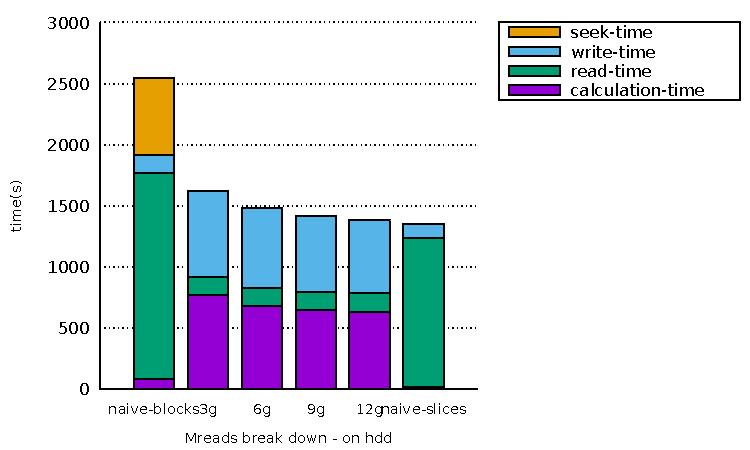
\includegraphics[width=0.45\columnwidth]{figures/benchmark-mreads/mreads-breakdown-hdd.pdf}
    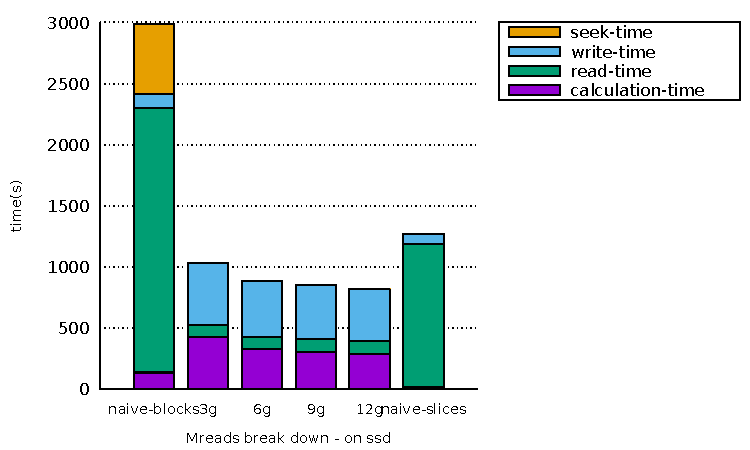
\includegraphics[width=0.45\columnwidth]{figures/benchmark-mreads/mreads-breakdown-ssd.pdf}
    \caption{Multiple reads}
  \end{subfigure}
  \caption{Breakdown of total merge times. Left column: HDD. Right column: SSD.}
  \label{fig:breakdowns-ssd}
  % Gnuplot file: scripts/experiment/compare_breakdown_errbar.gnuplot
\end{figure}


\subsubsection{Split time}

The number of seeks for Clustered writes and Multiple writes were
identical to the ones in Clustered reads and Multiple reads. \todo{Check
  that.} The total split time by algorithm is shown in
Figure~\ref{fig:split-time} and the breakdown by read, write, seek and
overhead time is in Figure~\ref{fig:breakdowns-ssd-split}. \todo{comment on the figures when results are available. Split time looks slightly longer than merge time.}

\begin{figure}[h]
  \centering
  \includegraphics[width=\columnwidth]{figures/total-split-time-hdd.pdf}\\
  \includegraphics[width=\columnwidth]{figures/total-split-time-ssd.pdf}
  \hfill
  \caption{Split time by algorithm. Top: HDD. Bottom: SSD. Each
    algorithm is represented with a different color. Averages over 5
    repetitions. Error bars show $\pm$ 1 standard deviation. }
  % Gnuplot file: scripts/experiment/split_and_merge_total_time.gnuplot
\label{fig:split-time}
\end{figure}

\begin{figure}
  \begin{subfigure}[b]{\columnwidth}
    \includegraphics[width=0.45\columnwidth]{figures/benchmark-buff-slices/buff-slices-breakdown-hdd-split.pdf}
    \includegraphics[width=0.45\columnwidth]{figures/benchmark-buff-slices/buff-slices-breakdown-ssd-split.pdf}
    \caption{Buffered slices}
  \end{subfigure}
  \begin{subfigure}[b]{\columnwidth}
    \includegraphics[width=0.45\columnwidth]{figures/benchmark-cwrites/cwrites-breakdown-hdd.pdf}
    \includegraphics[width=0.45\columnwidth]{figures/benchmark-cwrites/cwrites-breakdown-ssd.pdf}
    \caption{Clustered writes}
  \end{subfigure}
  \begin{subfigure}[b]{\columnwidth}
    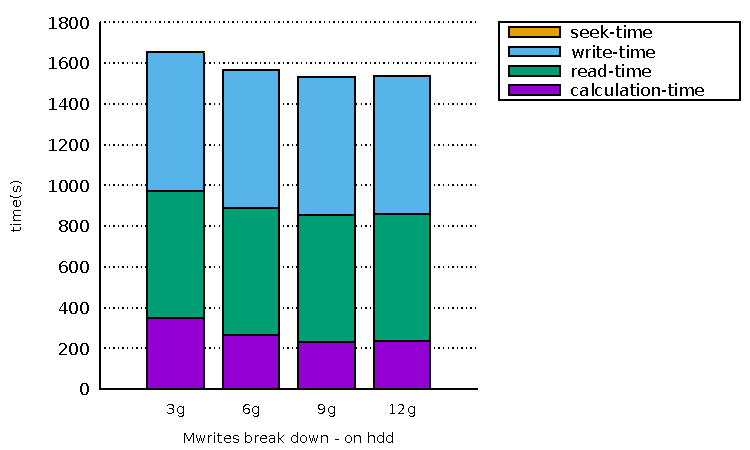
\includegraphics[width=0.45\columnwidth]{figures/benchmark-mwrites/mwrites-breakdown-hdd.pdf}
    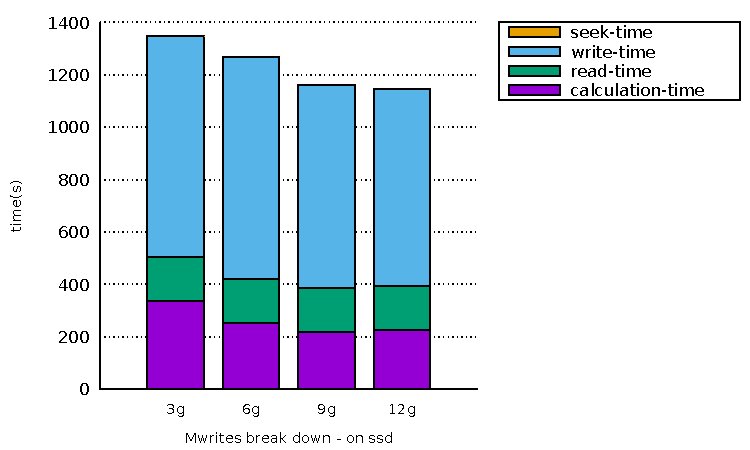
\includegraphics[width=0.45\columnwidth]{figures/benchmark-mwrites/mwrites-breakdown-ssd.pdf}
    \caption{Multiple writes}
  \end{subfigure}
  \caption{Breakdown of total split times. Left column: HDD. Right column: SSD.}
  \label{fig:breakdowns-ssd-split}
  % Gnuplot file: scripts/experiment/compare_breakdown_errbar.gnuplot
\end{figure}

\subsection{Compression}

Naive blocks, naive slices, cluster reads and multiple reads at 3, 6,
9, 12, 16GB, on SSD, with on-the-fly compression (graph will also show
without compression (previous results)) for comparison.

Expected result: Compression speeds up Multiple reads. It speeds up
Clustered reads to a smaller extent since Cluster reads still have to
seek in the reconstructed image. \todo{finish that up when the data is
  available}

\section{Discussion}
\label{sec:discussion}

% Problem solved!
Clustered reads and multiple reads are able to reduce to a negligible
amount the overall seek time required to split or merge 3D blocks in a
high-resolution image where data is stored linearly. Both algorithms
performed equivalently on our benchmark and compared to the reference
configuration where slices are merged or split without seeking. Our
initial problem is solved.

% Library is available. 
% overall, multiple reads is recommended as default parameters for the
% library. Clustered reads could be useful in some cases. 

%Same algo works for blocks or slices.

% Several other factors might influence performance
I/O optimization is a holistic problem that is in practice highly
dependent on the hardware used, firmware, operating system, file
system and programming language. Caching occurs at various levels and
might always influence performance, potentially differently depending
on the split or merge algorithm used. In some disks, seek time greatly
varies with the seek distance, which would open the door to additional
opportunities for I/O optimization. Interactions between those
components might also result in performance differences particular to
a particular algorithm. To ensure the portability of our library
across systems and configurations, we focused on reducing the overall
number of seeks and ignored specific system configurations. We
demonstrated the performance of our methods on both an HDD and an SSD
disk, using state-of-the-art and widely used versions of Linux
(CentOS7) and file systems (XFS v4.5.0).

% File formats
In terms of file formats, our results demonstrate that simple imaging
formats may be split and merged without performance loss compared to
more complex formats that try to preserve spatial locality on disk,
for instance MINC 2.0 or the format based on space-filling curves
mentioned in~\cite{burns2013open}. This is of major interest in the
current open-science context since simpler formats favor data-sharing
and interoperability.  Moreover, our algorithms could potentially be
adapted to any split geometry, even though we demonstrated them on
slices and blocks only, while file formats inevitably assume a
particular geometry. For instance, the format in~\cite{burns2013open}
is not designed to naively split slices. However, we aimed to extract
all the blocks, whereas, ~\cite{burns2013open} aimed to extract a
single block from a large image. MINC 2.0 might also help with
on-the-fly compression.

% Compression
Due to the minimal number of seeks in the reconstructed image,
Multiple reads greatly benefit from on-the-fly compression. This is
not the case of Clustered reads, where compression has an important
overhead due to residual seeking in the reconstructed
image. Techniques such as z-indexing have been used to address this
limitation of the NiFTI format~\cite{rajna2015speeding} and could be
employed here too.

% Parallel algorithms
High-resolution images are likely to be processed on computing
clusters, for instance using software from the Hadoop project, in
particular the Hadoop Distributed File
System~\cite{shvachko2010hadoop}. In this context parallel
split-and-merge algorithms would be beneficial, since the various
blocks of a large image could be uploaded to different disks
concurrently. In the same vein, ``re-spliting'' algorithms would be
beneficial in case an image already split needs to be split in a
different geometry. Clustered reads and multiple reads could be used
as starting points for such algorithms.

Our \texttt{sam} library is available at
\url{https://github.com/big-data-lab-team/sam}, under MIT license.

% Ideas for the future: measure the actual amount of consumed memory.

\section*{Acknowledgment}
We warmly thank Lindsay B. Lewis and Claude Lepage for helping us with
Big~Brain, Greg Kiar for useful discussion about the Open Connectome
Data Cluster and Pierre Bellec for discussions about MINC.

\bibliographystyle{IEEEtran}
\bibliography{IEEEabrv,biblio.bib}

\end{document}
